\documentclass[a4paper,10pt]{article}
\usepackage[utf8]{inputenc}
\usepackage{amsmath}
\usepackage{graphicx}
\usepackage{amsthm}
\usepackage{amsfonts}
\usepackage{dsfont}
\usepackage{pdfpages}
\usepackage{bm}
\usepackage{fontspec}
\usepackage{textcomp, xspace}

\usepackage{float}
\restylefloat{table}

\title{Guidelines and Conventions}
\author{Mikael Hedberg}

\begin{document}
	
\maketitle

\section{Layer Memory Layout}
When designing the architecture of the CNN, one of the goals was being able to support extremely large networks with as good performance as possible. For example, when back propagating a convolutional layer, you need either to add zero padding around the unit, or a bunch of conditional statements in the code that emulates zero padding. The latter is hard to maintain in the long run. For GPUs, it's always an bad idea to rely heavily on branching since the instruction set is executed simultaneously over a warp (or wavefront). Furthermore, allowing for padding and memory offsets, we have greater flexibility to align the memory for either 1) optimized memory access for GPUs or 2) vectorization for CPUs. The decision was taken to impose the below memory model that must be handled by the layers.

\begin{figure}[H]
	\centering
	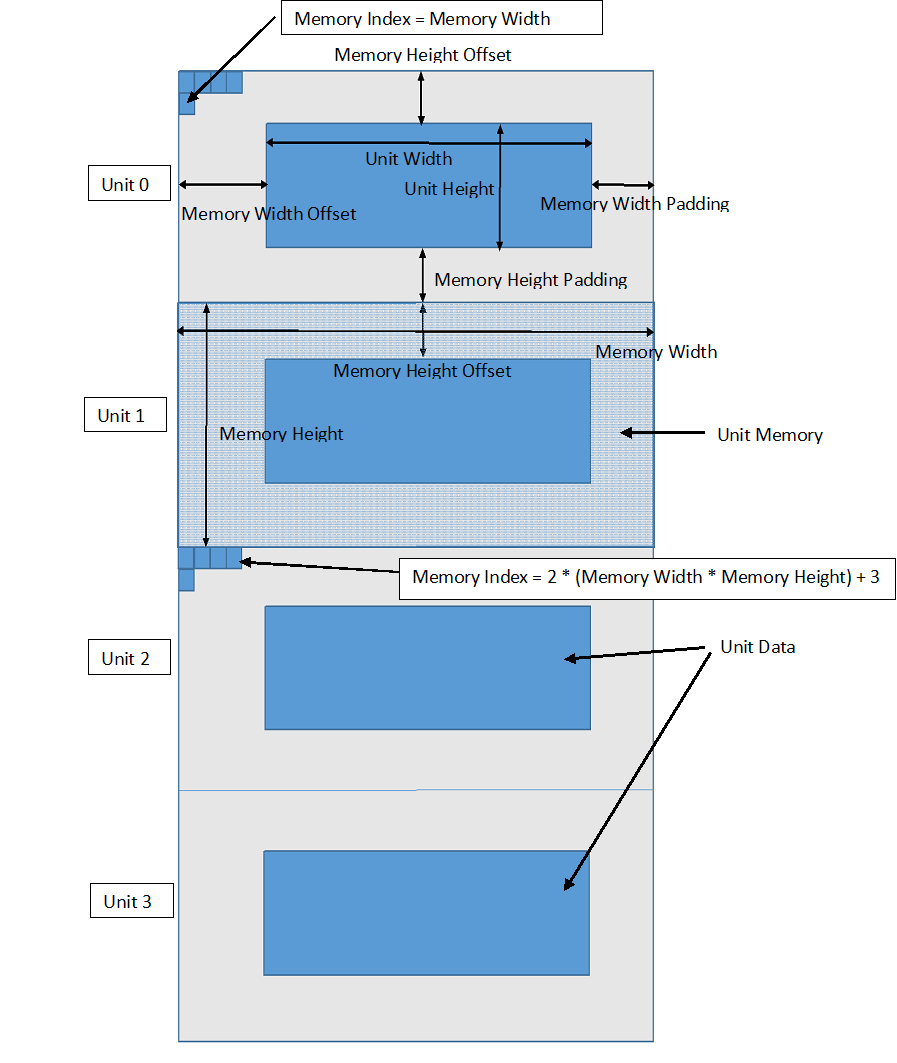
\includegraphics[scale=0.6]{MemoryLayoutWithDescription}
	\caption{Image showing the memory layout of a BLOB that is shared between layers. This memory layout will allow for maximum flexibility for the layers to try find an optimized layout for their particular problem. Since we impose that every layer must handle this layout, we will also avoid unnecessary memory copies that may or may not require an additional kernel call.}
	\label{fig:convNet}
\end{figure}

Before deducing the equations needed for memory access, the following variable conventions are imposed when dealing with memory access:
\begin{table}[H]
	\centering
	\footnotesize
	\hspace*{-3cm}\begin{tabular}{|l | l| l|}
		\hline
		\textbf{Name} & \textbf{Variable name} & \textbf{Macro name} \\
		\hline
		Unit offset & \textlangle description\textrangle UnitOffset & \textlangle DESCRIPTION\textrangle\_UNIT\_OFFSET \\
		\hline
		Number of units & \textlangle description\textrangle UnitCount & \textlangle DESCRIPTION\textrangle\_UNIT\_COUNT \\
		\hline
		Unit padding & \textlangle description\textrangle UnitPadding & \textlangle DESCRIPTION\textrangle\_UNIT\_PADDING \\
		\hline
		Number of memory units & \textlangle description\textrangle UnitMemoryCount & \textlangle DESCRIPTION\textrangle\_UNIT\_MEMORY\_COUNT \\
		\hline
		Unit data width & \textlangle description\textrangle UnitWidth & \textlangle DESCRIPTION\textrangle\_UNIT\_WIDTH \\
		\hline
		Unit data height & \textlangle description\textrangle UnitHeight & \textlangle DESCRIPTION\textrangle\_UNIT\_HEIGHT \\
		\hline
		Unit data height * width & \textlangle description\textrangle UnitElements & \textlangle DESCRIPTION\textrangle\_UNIT\_ELEMENTS \\
		\hline
		Unit memory width & \textlangle description\textrangle UnitMemoryWidth & \textlangle DESCRIPTION\textrangle\_UNIT\_MEMORY\_WIDTH \\
		\hline
		Unit memory height & \textlangle description\textrangle UnitMemoryHeight & \textlangle DESCRIPTION\textrangle\_UNIT\_MEMORY\_HEIGHT \\
		\hline
		Unit memory height * width & \textlangle description\textrangle UnitMemoryElements & \textlangle DESCRIPTION\textrangle\_UNIT\_MEMORY\_ELEMENTS \\
		\hline
		Unit memory width padding & \textlangle description\textrangle UnitMemoryWidthPadding & \textlangle DESCRIPTION\textrangle\_UNIT\_MEMORY\_WIDTH\_PADDING \\
		\hline
		Unit memory height padding & \textlangle description\textrangle UnitMemoryHeightPadding & \textlangle DESCRIPTION\textrangle\_UNIT\_MEMORY\_HEIGHT\_PADDING \\
		\hline
		Unit memory width offset & \textlangle description\textrangle UnitMemoryWidthOffset & \textlangle DESCRIPTION\textrangle\_UNIT\_MEMORY\_WIDTH\_OFFSET \\
		\hline
		Unit memory height offset & \textlangle description\textrangle UnitMemoryHeightOffset & \textlangle DESCRIPTION\textrangle\_UNIT\_MEMORY\_HEIGHT\_OFFSET \\
		\hline
	\end{tabular}
	\caption{A table showing the conventions for the variables describing the memory BLOB.}
\end{table}

When accessing this memory inside a kernel, the actual data units and the data units used inside the kernel do not necessarily align. For example, when back-propagating from a perceptron layer to a convolution layer, the convolution layer would require that you have at least some padding around every unit so that the rotated convolution kernel may be applied directly. This means that the data width for the convolution layer, inside the kernel, is $2 * (filterDimension - 1)$ larger than the actual data width outside the kernel. The convolution layer must here assure that the offset / padding is set to zeros. Furthermore, some hardware could require that the amount of global work units is a multiple of 8 in order to use vectorization. In this case a sufficient amount of padding is added and some "dummy" calculations are made on the padding. \\

In order to assure stability throughout the development of the kernels, we will also require the following conventions for global and local work units. 

\begin{table}[H]
	\centering
	\normalsize
	\begin{tabular}{|l | l| l|}
		\hline
		\textbf{Name} & \textbf{Variable name} & \textbf{Macro name} \\
		\hline
		Third global dimension size & globalUnits & GLOBAL\_UNITS \\
		\hline
		Second global dimension size & globalHeight & GLOBAL\_HEIGHT \\
		\hline
		First global dimension size & globalWidth & GLOBAL\_WIDTH \\
		\hline
		Third local dimension size & localUnits & LOCAL\_UNITS \\
		\hline
		Second local dimension size & localHeight & LOCAL\_HEIGHT \\
		\hline
		First local dimension size & localWidth & LOCAL\_WIDTH \\
		\hline
	\end{tabular}
	\caption{A table showing the conventions for the variables determining the global and local work sizes.}
\end{table}

Every other variable defined needed for successful kernel execution should follow the above guidelines. The equations determining global memory access is given by:
\begin{gather*}
x - widthIndex\\
y - heightIndex\\
z - unitIndex\\ \\
index = x + \langle DESCRIPTION\rangle\_UNIT\_MEMORY\_WIDTH\_OFFSET + \\
\langle DESCRIPTION\rangle\_UNIT\_MEMORY\_WIDTH * ( \\
 \langle DESCRIPTION\rangle\_UNIT\_MEMORY\_HEIGHT\_OFFSET + y) + \\
  \langle DESCRIPTION\rangle\_UNIT\_MEMORY\_ELEMENTS *( \\
  \langle DESCRIPTION\rangle\_UNIT\_OFFSET + z)
\end{gather*}

It's important to note that if you need to access an element inside a loop, you normally don't need to perform the entire calculating. It's enough to cache all the previous x,y,z values and simply perform a single addition inside the inner loop. Furthermore, for GPUs, the most important performance bottleneck lies in the memory access. This means that if you are using a memory access pattern that require a lot of arithmetic, but allows for better coalescing, then use it!

\appendix

\end{document}